\subsection{Errore 404}
L'errore 404 si verifica quando i link sono "rotti" (non esistono più). In questi casi, la cosa migliore da fare è dare altre scelte possibili all'utente, inserire una search box  e giocare sull'ironia dell'accaduto, per esempio con un’immagine divertente. Il fatto che ci si imbatta nella pagina 404 è un’esperienza negativa per l’utente, utile è dunque cercare di migliorare la situazione giocando sull'ironia della cosa, in modo tale che l’utente ne esca non con l’idea che ha perso tempo, ma che ha fatto una pausa da quello che stava cercando.  \\
Il sito ha optato per gestire l'errore eventuale come si vede nella \hyperref[img5]{Figura \ref{img5}} a destra con una barra di ricerca e una frase in inglese. Tuttavia mancano quelli che potrebbero essere dei suggerimenti per la prossima navigazione, eventuali frasi che suscitino interesse o la semplice ed ironica immagine dinamica che rilassa i timer dell'utente.
\begin{figure}[H]
	\centering
	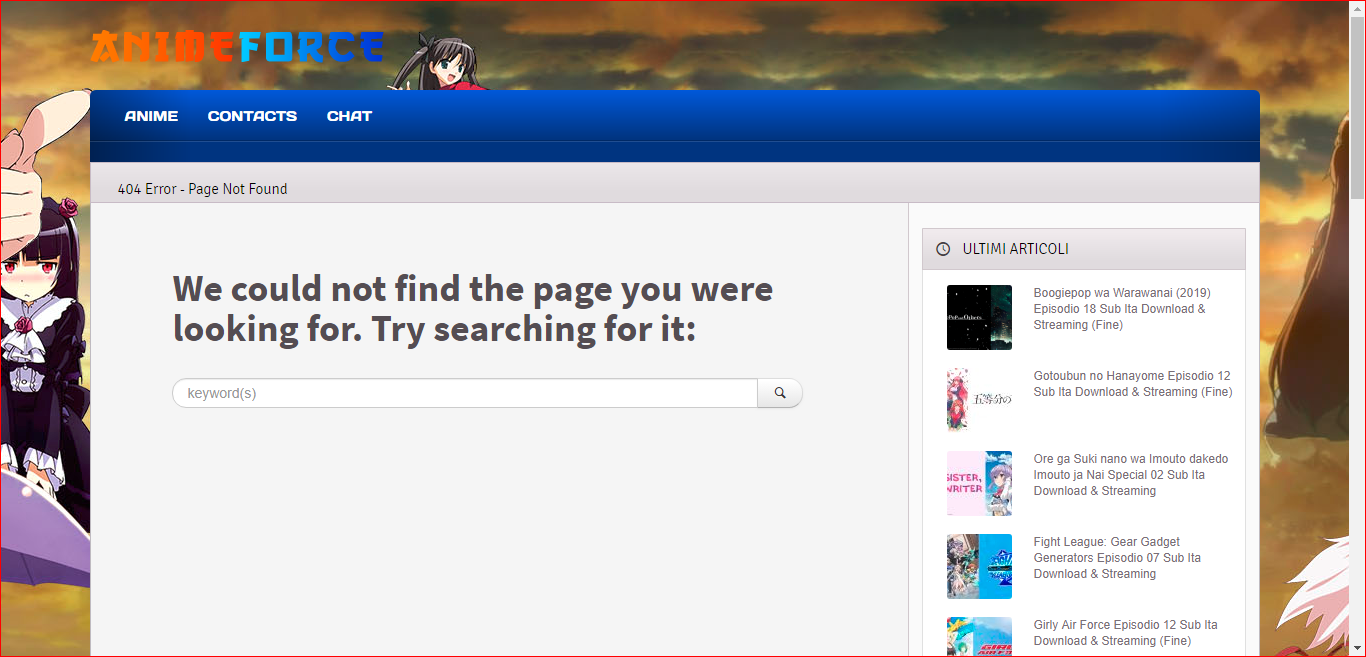
\includegraphics[width=1\textwidth]{img/Errore404.png}
	\caption{Menù} 
	\label{img5} 
\end{figure}